% Options for packages loaded elsewhere
\PassOptionsToPackage{unicode}{hyperref}
\PassOptionsToPackage{hyphens}{url}
%
\documentclass[
  italian,
]{article}
\usepackage{lmodern}
\usepackage{setspace}
\usepackage{amssymb,amsmath}
\usepackage{ifxetex,ifluatex}
\ifnum 0\ifxetex 1\fi\ifluatex 1\fi=0 % if pdftex
  \usepackage[T1]{fontenc}
  \usepackage[utf8]{inputenc}
  \usepackage{textcomp} % provide euro and other symbols
\else % if luatex or xetex
  \usepackage{unicode-math}
  \defaultfontfeatures{Scale=MatchLowercase}
  \defaultfontfeatures[\rmfamily]{Ligatures=TeX,Scale=1}
\fi
% Use upquote if available, for straight quotes in verbatim environments
\IfFileExists{upquote.sty}{\usepackage{upquote}}{}
\IfFileExists{microtype.sty}{% use microtype if available
  \usepackage[]{microtype}
  \UseMicrotypeSet[protrusion]{basicmath} % disable protrusion for tt fonts
}{}
\makeatletter
\@ifundefined{KOMAClassName}{% if non-KOMA class
  \IfFileExists{parskip.sty}{%
    \usepackage{parskip}
  }{% else
    \setlength{\parindent}{0pt}
    \setlength{\parskip}{6pt plus 2pt minus 1pt}}
}{% if KOMA class
  \KOMAoptions{parskip=half}}
\makeatother
\usepackage{xcolor}
\IfFileExists{xurl.sty}{\usepackage{xurl}}{} % add URL line breaks if available
\IfFileExists{bookmark.sty}{\usepackage{bookmark}}{\usepackage{hyperref}}
\hypersetup{
  pdftitle={MUSIC vs ESPRIT},
  pdfauthor={Andrea Feletto},
  pdflang={it-IT},
  hidelinks,
  pdfcreator={LaTeX via pandoc}}
\urlstyle{same} % disable monospaced font for URLs
\usepackage{graphicx}
\makeatletter
\def\maxwidth{\ifdim\Gin@nat@width>\linewidth\linewidth\else\Gin@nat@width\fi}
\def\maxheight{\ifdim\Gin@nat@height>\textheight\textheight\else\Gin@nat@height\fi}
\makeatother
% Scale images if necessary, so that they will not overflow the page
% margins by default, and it is still possible to overwrite the defaults
% using explicit options in \includegraphics[width, height, ...]{}
\setkeys{Gin}{width=\maxwidth,height=\maxheight,keepaspectratio}
% Set default figure placement to htbp
\makeatletter
\def\fps@figure{htbp}
\makeatother
\setlength{\emergencystretch}{3em} % prevent overfull lines
\providecommand{\tightlist}{%
  \setlength{\itemsep}{0pt}\setlength{\parskip}{0pt}}
\setcounter{secnumdepth}{-\maxdimen} % remove section numbering
\usepackage{siunitx}
\usepackage{listings}

\definecolor{codegreen}{rgb}{0,0.6,0}
\definecolor{codegray}{rgb}{0.5,0.5,0.5}
\definecolor{codepurple}{rgb}{0.58,0,0.82}
\definecolor{backcolour}{rgb}{0.95,0.95,0.92}

\lstdefinestyle{mystyle}{
    backgroundcolor=\color{backcolour},   
    commentstyle=\color{codegreen},
    keywordstyle=\color{magenta},
    numberstyle=\tiny\color{codegray},
    stringstyle=\color{codepurple},
    basicstyle=\ttfamily\footnotesize,
    breakatwhitespace=false,         
    breaklines=true,                 
    captionpos=b,                    
    keepspaces=true,                 
    numbers=left,                    
    numbersep=5pt,                  
    showspaces=false,                
    showstringspaces=false,
    showtabs=false,                  
    tabsize=2
}
\ifxetex
  % Load polyglossia as late as possible: uses bidi with RTL langages (e.g. Hebrew, Arabic)
  \usepackage{polyglossia}
  \setmainlanguage[]{italian}
\else
  \usepackage[shorthands=off,main=italian]{babel}
\fi
\ifluatex
  \usepackage{selnolig}  % disable illegal ligatures
\fi
\newlength{\cslhangindent}
\setlength{\cslhangindent}{1.5em}
\newlength{\csllabelwidth}
\setlength{\csllabelwidth}{3em}
\newenvironment{CSLReferences}[3] % #1 hanging-ident, #2 entry sp
 {% don't indent paragraphs
  \setlength{\parindent}{0pt}
  % turn on hanging indent if param 1 is 1
  \ifodd #1 \everypar{\setlength{\hangindent}{\cslhangindent}}\ignorespaces\fi
  % set line spacing
  % set entry spacing
  \ifnum #2 > 0
  \setlength{\parskip}{#3\baselineskip}
  \fi
 }%
 {}
\usepackage{calc} % for \widthof, \maxof
\newcommand{\CSLBlock}[1]{#1\hfill\break}
\newcommand{\CSLLeftMargin}[1]{\parbox[t]{\maxof{\widthof{#1}}{\csllabelwidth}}{#1}}
\newcommand{\CSLRightInline}[1]{\parbox[t]{\linewidth}{#1}}
\newcommand{\CSLIndent}[1]{\hspace{\cslhangindent}#1}

\title{MUSIC vs ESPRIT}
\author{Andrea Feletto}
\date{}

\begin{document}
\maketitle

{
\setcounter{tocdepth}{3}
\tableofcontents
}
\setstretch{1.25}
\newpage

\hypertarget{qualituxe0-dei-sistemi-elettrici-di-potenza}{%
\section{Qualità dei Sistemi Elettrici di
Potenza}\label{qualituxe0-dei-sistemi-elettrici-di-potenza}}

Negli anni il numero di studi operati nell'area riguardante la qualità
nei sistemi elettrici di potenza è aumentato notevolmente
(\protect\hyperlink{ref-dsp-pqd}{M. H. J. Bollen 2006}). Questo è dovuto
principalmente all'impiego di nuove fonti di energia, diverse esigenze
del consumatore e alla liberalizzazione del settore energetico.

L'avvento di nuove fonti di energia rinnovabile, come impianti solari ed
eolici, porta con se alcune criticità dovute ai disturbi che queste
generano quando allacciate alla rete elettrica. L'interconnessione alla
rete elettrica di fonti di energia caratterizzate da una capacità
produttiva variabile nel tempo è infatti causa di disturbi come il
\emph{voltage swell} e il \emph{voltage dip}
(\protect\hyperlink{ref-effective-power-quality}{R. Dash 2018}). Lo
standard \emph{IEEE 1159} definisce questi due disturbi
(\protect\hyperlink{ref-ieee-1159}{Board 1995}) rispettivamente come un
aumento e un calo di tensione per un tempo inferiore al minuto.

L'utilizzo di inverters, al fine di convertire la corrente continua
generata dai pannelli solari e dalle turbine eoliche in corrente
alternata, causa l'inserimento di armoniche e inter-armoniche nella
rete, dovute alla natura non lineare di questi dispositivi
(\protect\hyperlink{ref-impact-inverters}{J. Yaghoobi 2020}).

Un'altra fonte di disturbi armonici e inter-armonici sono i dispositivi
non lineari, necessari al funzionamento dei dispositivi alimentati in
corrente continua in uso al giorno d'oggi. In ambito civile infatti, a
differenza dei contesti industriali, buona parte del fabbisogno
energetico domestico è speso in illuminazione, riscaldamento, aria
condizionata e dispositivi elettronici, come personal computers e
televisori (\protect\hyperlink{ref-losses-cables}{F. L. Tofoli, s.d.}).
Nell'ultimo secolo si è quindi osservato un forte peggioramento della
qualità della rete, provocato da un uso sempre maggiore di inverters,
raddrizzatori di tensione e motori elettrici.

Una distorsione armonica è la presenza nel segnale di componenti
armoniche con frequenze multiple della frequenza di rete \(f_0\), mentre
una distorsione inter-armonica è caratterizzata da frequenze che deviano
da quelle armoniche. Le problematiche dovute a questi tipi di disturbo
sono molteplici.

Una ricerca svolta dall'\emph{Institute of Electrical and Electronics
Engineers} ha studiato gli effetti delle armoniche ad alta frequenza sul
funzionamento dei trasformatori monofase. È stata individuata una
proporzionalità tra le dissipazioni dovute a correnti parassite e il
quadrato della frequenza dell'armonica considerata
(\protect\hyperlink{ref-transformer-harmonic-loss}{D. Yildirim 2000}).
Questo significa che un buon algoritmo di stima delle armoniche deve
essere in grado di individuare anche le frequenze più alte, in quanto
queste sono responsabili per la maggior parte delle dissipazioni di
questo tipo. Lo stesso Istituto ha svolto un ulteriore studio, il quale
dimostra che le perdite di carico nei cavi e nei trasformatori di un
impianto elettrico, dovute ad un'elevata presenza di armoniche, possono
essere sufficientemente alte da giustificare modifiche all'impianto,
come l'aumento della sezione dei cavi o l'installazione di condensatori
per il rifasamento (\protect\hyperlink{ref-losses-cables}{F. L. Tofoli,
s.d.}).

Al fine di caratterizzare l'entità dei disturbi armonici e
inter-armonici all'interno di un segnale elettrico di potenza, risulta
utile il concetto di \textbf{Distorsione Armonica Totale}, la quale,
note le componenti del segnale, si può calcolare come segue: \[
THD^2 = \frac{\sum_{k=2}^{K} V_k^2}{V_1^2}
\] Dove \(V_1\) è la tensione di linea e \(V_k\) è la tensione della
\(k\)-esima armonica. Il THD è quindi la percentuale di energia presente
nel segnale non dovuta alla componente fondamentale
(\protect\hyperlink{ref-dsp-pqd}{M. H. J. Bollen 2006}).

È importante precisare che i disturbi di tensione sono prodotti dal
generatore, mentre i disturbi di corrente sono causati dagli
utilizzatori. Tuttavia, se questi ultimi non vengono opportunamente
compensati, una volta raggiunta la sorgente provocano ulteriori disturbi
di tensione.

La liberalizzazione del mercato dell'energia ha delle notevoli
conseguenze nel campo della qualità dei segnali di potenza
(\protect\hyperlink{ref-power-quality-deregulation}{J. Arrillaga 2000}).
La necessità di aumentare i margini di guadagno porta le compagnie
operanti nel settore dell'energia a ridurre la manutenzione e lo
sviluppo dei sistemi di distribuzione. Ciò comporta un inevitabile
peggioramento della qualità. Inoltre, la ridotta cooperazione tra
società in concorrenza tra loro impatta negativamente lo sviluppo di
tecnologie e standards.

\hypertarget{algoritmi-per-la-stima-dei-disturbi-armonici}{%
\section{Algoritmi per la stima dei disturbi
armonici}\label{algoritmi-per-la-stima-dei-disturbi-armonici}}

Esistono numerosi algoritmi che permettono di stimare frequenza,
ampiezza e fase delle componenti sinusoidali di un segnale. Si noti che
non esiste un algoritmo adatto ad ogni contesto. Spesso infatti, la
precisione sulle misurazioni è correlata alla complessità
computazionale.

Il primo metodo basato sullo studio della matrice di covarianza è la
\emph{Pisarenko Harmonic Decomposition} (PHD)
(\protect\hyperlink{ref-pisarenko-single-tone}{K. W. Chan 2003}),
risalente al 1973 (\protect\hyperlink{ref-pisarenko-original}{Pisarenko
1973}). La PHD, basandosi sull'autovalore minore della matrice di
covarianza, e all'autovettore associato
(\protect\hyperlink{ref-pisarenko-stat-analysis}{Sakai 1984}), permette
di stimare le frequenza di una sinusoide addizionata a rumore bianco
gaussiano: \[
\hat{\omega} = cos^{-1} \left(
    \frac{r_2 + \sqrt{r_2^2 + 8 r_1^2}}{4 r_1}
\right)
\] dove \(r_k\) è la covarianza campionaria: \[
r_k = \frac{1}{N - k} \sum_{n=1}^{N-k} x(n) x(n + k)
\] Questo algoritmo permette la stima solamente dell'armonica principale
e non è quindi utile nello studio dei disturbi armonici.

L'algoritmo più usato è la \emph{Fast Fourier Transform} (FFT) che
permette di calcolare la \emph{Discrete Fourier Transform} (DFT)
(eq.~\ref{eq:dft}) di un segnale a tempo discreto di lunghezza finita
\(N\). \begin{equation}\protect\hypertarget{eq:dft}{}{
X[k] = \sum_{n=0}^{N-1} x[n] \, e^{-j \frac{2\pi}{N}kn}
}\label{eq:dft}\end{equation} È un algoritmo di tipo \emph{Divide and
Conquer} ed ha quindi una complessità asintotica
\(\mathcal{O}(N\log{}N)\)
(\protect\hyperlink{ref-fourier-alg-machine}{J. W. Cooley 1965}). È un
algoritmo veloce e di facile implementazione, ma ha molte limitazioni.

La risoluzione dello spettro generato è inversamente proporzionale alla
lunghezza del segnale campionato
(\protect\hyperlink{ref-alg-comp-quality}{P. M. Ramos 2009}) \[
\Delta f = \frac{1}{t_w}
\] dove \(t_w\) è la durata temporale del campionamento. Se il segnale
contiene armoniche la cui frequenza cambia nel tempo, \(t_w\) deve
essere sufficientemente piccolo da permettere una risoluzione temporale
che consenta di osservare la variazione delle frequenze. Questo però
implica una bassa risoluzione spettrale, la quale implica un notevole
errore sulla stima della frequenza.

La FFT soffre inoltre dell'effetto di \emph{spectral leakage}
(\protect\hyperlink{ref-fft-time-domain-window}{S. Rapuano 2007}). Se la
lunghezza del segnale non è tale da includere esclusivamente periodi
interi di ogni componente sinusoidale, lo spettro presenta errori di
frequenza, ampiezza e fase. Poiché non è possibile conoscere a priori la
lunghezza necessaria per non ottenere questo effetto, ogni applicazione
reale della FFT presenterà errori di misura dovuti al \emph{leakage}.

L'\emph{Interpolated Fast Fourier Transform} (IFFT) è un algoritmo
sviluppato al al fine di ottenere misurazioni precise di frequenza,
ampiezza e fase da segnali affetti da \emph{spectral leakage}
(\protect\hyperlink{ref-ifft-comp}{J. Schoukens 1992}). L'algoritmo è
basato sull'applicazione al segnale di una funzione finestra
opportunamente scelta (\protect\hyperlink{ref-ifft-original}{D. C. Rife
1970}). Due funzioni finestra spesso utilizzate sono la \emph{Hanning
window} (eq.~\ref{eq:hanning-window}) e la \emph{Rife-Vincent window}.
\begin{equation}\protect\hypertarget{eq:hanning-window}{}{
w[n] = sin^2 \left( \frac{\pi n}{N} \right)
}\label{eq:hanning-window}\end{equation} Uno studio pubblicato dalla
IEEE (\protect\hyperlink{ref-ifft-comp}{J. Schoukens 1992}) ha
confrontato le prestazioni di queste due funzioni finestra. La
\emph{Hanning window} è risultata la scelta più adeguata per segnali con
un basso rapporto segnale/rumore (SNR) e dei quali non si hanno
informazioni sulle frequenze contenute.

Questo algoritmo è poco adatto all'analisi di segnali contenenti
armoniche o inter-armoniche vicine alla frequenza di rete e con ampiezza
simile. Queste possono infatti distorcere l'interpolazione dello spettro
risultante (\protect\hyperlink{ref-alg-comp-quality}{P. M. Ramos 2009}).

\begin{figure}
\hypertarget{fig:music-odd-even}{%
\centering
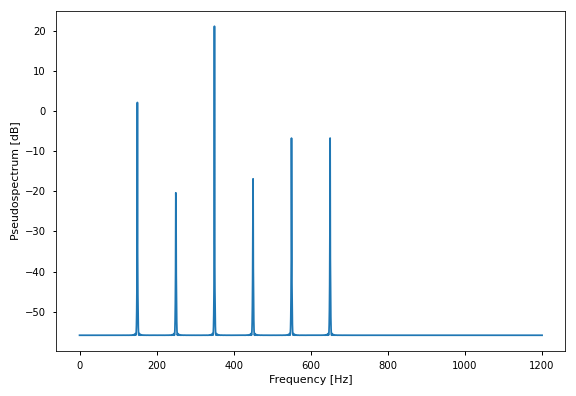
\includegraphics[width=0.6\textwidth,height=\textheight]{assets/music-odd-even.png}
\caption{Pseudospettro generato da MUSIC}\label{fig:music-odd-even}
}
\end{figure}

\emph{Multiple Signal Classification} (MUSIC) è un algoritmo basato
sull'analisi della matrice di autocorrelazione, in particolare sulla sua
decomposizione in autovettori
(\protect\hyperlink{ref-multiple-emitter-location}{Schmidt 1986}). MUSIC
prevede di ricavare uno pseudo-spettro (fig.~\ref{fig:music-odd-even})
stimando il sottospazio del rumore, e di ottenere le informazioni sulle
frequenze dai massimi locali. Al fine di stimare la matrice di
correlazione \(R\), una matrice \(\mathbf{V}\) viene costruita mediante
scorrimento di una finestra rettangolare larga \(M\) sul segnale
campionato di lunghezza \(N\). \[
R = \frac{1}{N} \mathbf{V}^t \, \mathbf{V}
\] La scelta di \(M\) influenza la precisione della misurazione. In
particolare \(M\) deve essere tale da far sì che una finestra includa
solamente periodi interi della componente principale
(\protect\hyperlink{ref-sliding-window-esprit}{Bollen 2008}).

Gli autovettori \(\mathbf{s}_i\) della matrice di autocorrelazione \(R\)
formano il sottospazio del segnale e il sottospazio del rumore.
Quest'ultimo è formato dagli autovettori associati agli \(M - K\)
autovalori minori. Le frequenze sono quindi stimate individuando i
picchi dello pseudo-spettro dato dal sottospazio del rumore: \[
P_{music} \left( e^{j \omega} \right) =
\frac{1}{\sum_{i=K+1}^{M} \left| \mathbf{e}^H \mathbf{s}_i  \right|^2}
\] dove \(\mathbf{e}^H\) è il vettore di \emph{steering} trasposto e
coniugato.

Il metodo ESPRIT, a differenza di MUSIC, sfrutta il sottospazio del
segnale (\protect\hyperlink{ref-dsp-pqd}{M. H. J. Bollen 2006}).
L'algoritmo permette di individuare la matrice diagonale di rotazione
\(\Phi\) (\protect\hyperlink{ref-esprit-original}{R. Roy 1989}), i cui
elementi sono gli esponenziali complessi di fase pari alle pulsazioni
delle \(K\) componenti sinusoidali del segnale. \[
\Phi = diag \left\{ e^{j \omega_1}, \, \ldots, \, e^{j \omega_K} \right\}
\] Una matrice \(\Psi\), i cui autovettori coincidono con gli elementi
sulla diagonale di \(\Phi\), viene stimata grazie alla decomposizione ai
valori singolari (SVD) della matrice \(\mathbf{V}\) usata in MUSIC.
ESPRIT permette anche la stima del decadimento (se presente) delle
sinusoidi modellando opportunamente i gli esponenziali complessi: \[
\Phi = diag \left\{
    e^{-\beta_1 + j \omega_1}, \, \ldots, \, e^{- \beta_K + j \omega_K}
\right\}
\] dove \(\beta_k\) è il decadimento della \(k\)-esima armonica.

Spesso la componente principale del segnale ha un'ampiezza uno o due
ordini di grandezza superiore a quella delle componenti armoniche. In
questi casi è quindi necessario applicare un filtro passa-alto al
segnale prima di stimarne i disturbi armonici. La sproporzione nel
contenuto energetico comporta infatti un aumento dell'errore di stima
(\protect\hyperlink{ref-dsp-pqd}{M. H. J. Bollen 2006}).

Una diversa rappresentazione matematica del segnale è quella in spazio
di stato. Nel caso di un segnale stazionario, questo può essere
rappresentato da due equazioni (\protect\hyperlink{ref-dsp-pqd}{M. H. J.
Bollen 2006}): \[
\begin{cases}
\mathbf{x}[n] = A \, \mathbf{x}[n-1] + \mathbf{w}[n] \\
\mathbf{z}[n] = C \, \mathbf{x}[n] + \mathbf{v}[n]
\end{cases}
\] dove \(\mathbf{x}\) è il vettore di stato, \(A\) la matrice di
transizione, \(\mathbf{w}\) il vettore del rumore, \(\mathbf{z}\) il
vettore delle misurazioni, \(C\) la matrice di misurazione e
\(\mathbf{v}\) il vettore del rumore dovuto alla misurazione.

Sfruttando questa rappresentazione è possibile stimare il contenuto
armonico (e altri tipi di disturbi) applicando il filtro di Kalman.
L'algoritmo si basa sulla minimizzazione dell'errore \(\mathbf{e}\)
nella stima del vettore di stato \(\mathbf{x}\)
(\protect\hyperlink{ref-state-est-kalman}{I. M. Moreno 2020}). \[
\mathbf{e}[n] = \mathbf{x}[n] - \hat{\mathbf{x}}[n]
\] L'applicazione del filtro prevede la conoscenza a priori delle
pulsazioni \(\omega_k\) delle quali si vuole conoscere ampiezza e fase.
Se è possibile assumere la sola presenza di armoniche, è sufficiente
stimare un valore di \(K\) sufficientemente alto da verificare
l'assunzione che i rumori \(\mathbf{w}\) e \(\mathbf{v}\) siano
gaussiani a media nulla. Nel caso di presenza di inter-armoniche non è
realisticamente possibile assumere i valori delle pulsazioni, il che
rende il filtro di Kalman inadatto a misurazioni di questo tipo.

\hypertarget{stima-di-armoniche-e-interarmoniche}{%
\section{Stima di Armoniche e
Interarmoniche}\label{stima-di-armoniche-e-interarmoniche}}

\hypertarget{modello-sinusoidale}{%
\subsection{Modello Sinusoidale}\label{modello-sinusoidale}}

Ogni segnale a tempo discreto \(v[n]\) ottenuto da una rete elettrica
può essere espresso come la sovrapposizione di \(K\) componenti
sinusoidali, più una componente di rumore. \[
v[n] = s[n] + w[n] = \sum_{k=1}^K s_k[n] + w[n]
\] Le componenti sinusoidali sono caratterizzate dall'ampiezza
\(a_k \geq 0\), dalla fase \(\phi_k \in [-\pi, \pi]\) e dalla pulsazione
\(\omega_k\). \[
s_k[n] = a_k \, cos \left( n \omega_k + \phi_k \right)
\] Le componenti \(s_k[n]\) sono chiamate \textbf{armoniche} quando la
loro pulsazione è un multiplo della pulsazione fondamentale
\(\omega_0\), altrimenti sono dette \textbf{interarmoniche}.

La \(\tilde{k}\)-esima armonica ha pulsazione
\(\omega_k = 2 \tilde{k} \pi f_0\). Si noti che le frequenze sono
normalizzate rispetto alla frequenza di campionamento secondo la
relazione \(f_k = \tilde{f_k} / f_s\), dove \(\tilde{f_k}\) è la
frequenza in \(\si{\hertz}\) e \(f_s\) è la frequenza di campionamento.
Pertanto, se viene rispettato il Teorema del Campionamento di
Nyquist-Shannon: \[
f_c > 2 \, max\{f_k\}
\] ne deriva che \(\omega_k \in \left[ -\pi, \pi \right]\).

La \(0\)-esima armonica, avendo pulsazione nulla, è detta componente di
corrente continua e il suo valore di tensione è
\(V_{DC} = a_0 \, cos(\phi_0)\). L'armonica fondamentale è detta invece
componente di potenza ed ha pulsazione
\(\omega_0 = \tau \tilde{f}_0 / f_c\) e ampiezza
\(a_0 = \sqrt{2} \, V_{rms}\), dove \(\tilde{f}_0\) è la frequenza della
rete e \(V_{rms}\) è la tensione efficace di fase.

\hypertarget{modello-armonico}{%
\subsection{Modello Armonico}\label{modello-armonico}}

Il segnale \(v[n]\) può essere espresso anche sotto forma di
esponenziali complessi. La \(k\)-esima componente ha quindi la seguente
forma: \[
v_k[n] = A_k e^{j \phi_k} e^{j n \omega_k}
\]

Due campioni successivi della componente \(v_k[n]\) sono legati da uno
sfasamento pari alla sua pulsazione \(\omega_k\). \[
v_k[n+1] = v_k[n] e^{j \omega_k}
         = A_k e^{j \phi_k} e^{j (n+1) \omega_k}
\]

\hypertarget{riduzione-dimensionale-del-segnale}{%
\subsection{Riduzione Dimensionale del
Segnale}\label{riduzione-dimensionale-del-segnale}}

Dato un segnale \(v[n]\) di lunghezza \(L = N + M - 1\), si definisce il
vettore dei campionamenti \(\mathbf{v}[n]\) come la finestra di ampiezza
\(M\) da \(v[n]\) a \(v[n + M - 1]\). Il vettore \(\mathbf{v}[n]\) è
quindi un campionamento \(M\)-dimensionale del segnale.

Si costruisce (\protect\hyperlink{ref-dsp-pqd}{M. H. J. Bollen 2006}) la
matrice \(\mathbf{V}\), di dimensioni \(N \times M\), ponendo sulle
righe i vettori di campionamento \(\mathbf{v}[n]\) \[
\mathbf{V} =
\begin{bmatrix}
    \mathbf{v}^t[0] \\
    \vdots \\
    \mathbf{v}^t[N - 1]
\end{bmatrix}
=
\begin{bmatrix}
v[0]   & \dots  & v[M - 1] \\
\vdots & \ddots & \vdots   \\
v[N - 1] & \dots & v[N + M - 2]
\end{bmatrix}
\] ottenendo quindi una sequenza di \(N\) misurazioni
\(M\)-dimensionali.

Assumendo che il rumore \(w[n]\), e di conseguenza il segnale \(v[n]\),
abbia media nulla, si osserva che migliore è la scelta di \(M\), tale
che ogni vettore di campionamento \(\mathbf{v}[n]\) includa periodi
interi di ogni armonica, più la media di \(\mathbf{v}[n]\) tende ad
annullarsi.

Ciò permette di stimare la matrice di correlazione campionaria
\(\mathbf{R}_{kl}\) \[
\hat{\mathbf{R}}_{kl} = \mathit{E} \left\{
    \mathbf{v}^{(k)} \circ \mathbf{v}^{(l)}
\right\}
  = \frac{1}{N} \, \mathbf{v}^{(k)} \cdot \mathbf{v}^{(l)}
\] , dove \(\mathbf{v}^{(k)}\) è la \(k\)-esima colonna di
\(\mathbf{V}\). Riscrivendo l'equazione in forma matriciale si ottiene:
\[
\hat{\mathbf{R}} = \frac{1}{N} \, \mathbf{V}^t \, \mathbf{V}
\]

\hypertarget{algoritmo-music}{%
\subsection{Algoritmo MUSIC}\label{algoritmo-music}}

Per il principio della sovrapposizione degli effetti la matrice di
correlazione del segnale \(\mathbf{R}\) può essere espressa come somma
della matrici di correlazione \(\mathbf{R}_s\) e \(\mathbf{R}_n\) dovute
rispettivamente alle componenti armoniche e al rumore.

Assumendo che il rumore sia di natura gaussiana con varianza
\(\sigma_w^2\), la sua matrice di correlazione vale: \[
\mathbf{R}_w = \sigma_w^2 I
\] dove \(I\) è la matrice identità di dimensione \(M \times M\) e
\(\sigma_w^2\) coincide con la potenza del rumore.

\hypertarget{algoritmo-esprit}{%
\subsection{Algoritmo ESPRIT}\label{algoritmo-esprit}}

Isolando le componenti di segnale e di rumore, utilizzando una notazione
analoga a quella del vettore dei campionamenti, si ha:
\begin{equation}\protect\hypertarget{eq:sig:sampleform}{}{
\mathbf{v}[n] = \sum_{k=1}^K \mathbf{s}_k[n] + \mathbf{w}[n]
}\label{eq:sig:sampleform}\end{equation} Studiando il contributo
\(\mathbf{s}_k[n]\) della \(k\)-esima componente armonica e applicando
le proprietà del modello armonico, è possibile esprimere ogni elemento
\(\mathbf{s}_{k,i}[n]\) in funzione di \(s_k[n]\): \[
\mathbf{s}_{k,i}[n] = s_k[n + i] = s_k[n] e^{j i \omega_k}
\] E riscrivendo \(\mathbf{s}_k[n]\) in forma vettoriale si ottiene: \[
\mathbf{s}_{k}[n] = s_k[n]
\begin{bmatrix}
    1 \\
    e^{j \omega_k} \\
    \vdots \\
    e^{j (M-1) \omega_k}
\end{bmatrix} =
s_k[n] \, \mathbf{e}_k
\] dove \(\mathbf{e}_k\) è detto \emph{vettore steering}, il quale è
formato dagli sfasamenti successivi associati alla pulsazione
\(\omega_k\).

È quindi possibile riscrivere l'equazione
\{eq.~\ref{eq:sig:sampleform}\} come trasformazione lineare del vettore
delle ampiezze complesse \(\mathbf{A}\): \[
\mathbf{v}[n] = \mathbf{E} \Phi^n \mathbf{A} + \mathbf{w}[n]
\] dove \(\mathbf{E}\) è una matrice \(M \times K\) le cui \(k\)-esima
colonna è il vettore steering associato alla pulsazione \(\omega_k\) \[
\mathbf{E} = \left[ \mathbf{e}_1, \ldots, \mathbf{e}_K \right]
\] , \(\Phi\) è una matrice diagonale i cui elementi sono gli
esponenziali complessi associati alle \(K\) diverse pulsazioni \[
\Phi = diag \left\{ e^{j \omega_1}, \ldots, e^{j \omega_K} \right\}
\] mentre \(A\) è il vettore delle ampiezze complesse \[
\mathbf{A} = \begin{bmatrix}
    A_1 e^{j \phi_1} \\
    \vdots \\
    A_K e^{j \phi_K}
\end{bmatrix}
\]

\hypertarget{implementazione-in-python}{%
\section{Implementazione in Python}\label{implementazione-in-python}}

Diverse librerie sono state utilizzate per l'implementazione e la
visualizzazione degli algoritmi MUSIC e ESPRIT. La lettura e la
memorizzazione di dati tabulari è gestita da \emph{pandas}. \emph{numpy}
permentte invece la memorizzazione di array contigui in memoria,
garantendo ottime prestazioni di calcolo nonostante il livello di
astrazione. Le routines per i calcoli di algebra lineare e per la
localizzazione di massimi locali sono formite dalla libreria
\emph{scipy}. Per la visualizzazione è stata usata \emph{matplotlib}.

Per garantire la riproducibilità delle stime, il generatore di numeri
pseudo-casuali incluso in \emph{numpy} è stato inizializzato con un seme
scelto arbitrariamente.

\begin{lstlisting}[language=Python]
from math import tau

import matplotlib.pyplot as plt
import numpy as np
import pandas as pd
import scipy as sp
import scipy.linalg as LA
import scipy.signal as ss

from utils import *

plt.style.use('seaborn-notebook')
np.random.seed(293710966)
\end{lstlisting}

\newpage

\hypertarget{riferimenti}{%
\section*{Riferimenti}\label{riferimenti}}
\addcontentsline{toc}{section}{Riferimenti}

\hypertarget{refs}{}
\begin{CSLReferences}{1}{0}
\leavevmode\hypertarget{ref-ieee-1159}{}%
Board, IEEE Standards. 1995. {«{IEEE} 1159-1995 - {IEEE} Recommended
Practice for Monitoring Electric Power Quality»}.

\leavevmode\hypertarget{ref-sliding-window-esprit}{}%
Bollen, I. Y. H. Gu; M. H. J. 2008. {«Estimating interharmonics by using
sliding-window {ESPRIT}»}. \emph{{IEEE} Transactions on Power Delivery}
23: 13--23.
https://doi.org/\url{https://doi.org/10.1109/TPWRD.2007.911130}.

\leavevmode\hypertarget{ref-ifft-original}{}%
D. C. Rife, G. A. Vincent. 1970. {«Use of the discrete fourier transform
in the measurement of frequencies and levels of tones»}. \emph{The Bell
System Technical Journal} 49: 197--228.
https://doi.org/\url{https://doi.org/10.1002/j.1538-7305.1970.tb01766.x}.

\leavevmode\hypertarget{ref-transformer-harmonic-loss}{}%
D. Yildirim, E. F. Fuchs. 2000. {«Measured transformer derating and
comparison with harmonic loss factor \(F_{HL}\) approach»}. \emph{{IEEE}
Transactions on Power Delivery} 15: 186--91.
https://doi.org/\url{https://doi.org/10.1109/61.847249}.

\leavevmode\hypertarget{ref-losses-cables}{}%
F. L. Tofoli, A. de Oliveira, S. M. R. Sanhueza. s.d. {«On the Study of
Losses in Cables and Transformers in Nonsinusoidal Conditions»}.
\emph{{IEEE} Transaction on Power Delivery} 21: 971--78.
https://doi.org/\url{https://doi.org/10.1109/TPWRD.2006.870986}.

\leavevmode\hypertarget{ref-state-est-kalman}{}%
I. M. Moreno, R. C. Magaña, A. Medina. 2020. {«Enhanced harmonic state
estimation in unbalanced three-phase electrical grids based on the
Kalman filter and physical scale-down implementation»}.
\emph{International Journal of Electrical Power and Energy Systems} 123:
106243.
https://doi.org/\url{https://doi.org/10.1016/j.ijepes.2020.106243}.

\leavevmode\hypertarget{ref-power-quality-deregulation}{}%
J. Arrillaga, N. R. Watson, M. H. J. Bollen. 2000. {«Power Quality
Following Deregulation»}. \emph{Proceedings of the {IEEE}} 88: 246--61.
https://doi.org/\url{https://doi.org/10.1109/6.387140}.

\leavevmode\hypertarget{ref-ifft-comp}{}%
J. Schoukens, H. Van hamme, P. Pintelon. 1992. {«The Interpolated Fast
Fourier Transform: A Comparative Study»}. \emph{{IEEE} Transactions on
Instrumentation and Measurement} 41: 226--32.
https://doi.org/\url{https://doi.org/10.1109/19.137352}.

\leavevmode\hypertarget{ref-fourier-alg-machine}{}%
J. W. Cooley, J. W. Tukey. 1965. {«An Algorithm for the Machine
Calculation of Complex Fourier Series»}. \emph{Mathematics of
Computation} 19: 297--301.

\leavevmode\hypertarget{ref-impact-inverters}{}%
J. Yaghoobi, D. Martin, A. Alduraibi. 2020. {«Impact of high-frequency
harmonics (0--9 kHz) generated by grid-connected inverters on
distribution transformers»}. \emph{Electrical Power and Energy Systems}
122: 106--77.
https://doi.org/\url{https://doi.org/10.1016/j.ijepes.2020.106177}.

\leavevmode\hypertarget{ref-pisarenko-single-tone}{}%
K. W. Chan, H. C. So. 2003. {«An exact analysis of Pisarenko's
single-tone frequencyestimation algorithm»}. \emph{Signal Processing}
83: 685--90.
https://doi.org/\url{https://doi.org/10.1016/S0165-1684(02)00493-0}.

\leavevmode\hypertarget{ref-dsp-pqd}{}%
M. H. J. Bollen, I. Y. H. Gu. 2006. \emph{Signal Processing of Power
Quality Disturbances}. Wiley-{IEEE} Press.
\url{https://ieeexplore.ieee.org/servlet/opac?bknumber=5224658}.

\leavevmode\hypertarget{ref-alg-comp-quality}{}%
P. M. Ramos, A. C. Serra. 2009. {«Comparison of Frequency Estimation
Algorithms for Power Quality Assessment»}. \emph{Measurement} 42:
1312--17.
https://doi.org/\url{https://doi.org/10.1016/j.measurement.2008.04.013}.

\leavevmode\hypertarget{ref-pisarenko-original}{}%
Pisarenko, V. F. 1973. {«The Retrieval of Harmonics from a Covariance
Function»}. \emph{Geophysical Journal International} 33: 347--66.
https://doi.org/\url{https://doi.org/10.1111/j.1365-246X.1973.tb03424.x}.

\leavevmode\hypertarget{ref-effective-power-quality}{}%
R. Dash, S. C. Swain. 2018. {«Effective Power quality improvement using
Dynamic Activatecompensation system with Renewable grid interfaced
sources»}. \emph{Ain Shams Engineering Journal} 9: 2897--2905.
https://doi.org/\url{https://doi.org/10.1016/j.asej.2017.09.007}.

\leavevmode\hypertarget{ref-esprit-original}{}%
R. Roy, T. Kailath. 1989. {«{ESPRIT} - estimation of signal parameters
via rotational invariance techniques»}. \emph{{IEEE} Transactions on
Acoustics, Speech, and Signal Processing} 37: 984--95.
https://doi.org/\url{https://doi.org/10.1109/29.32276}.

\leavevmode\hypertarget{ref-fft-time-domain-window}{}%
S. Rapuano, F. J. Harris. 2007. {«An Introduction to FFT and Time Domain
Windows»}. \emph{{IEEE} Instrumentation and Measurement Magazine} 10:
32--44. https://doi.org/\url{https://doi.org/10.1109/MIM.2007.4428580}.

\leavevmode\hypertarget{ref-pisarenko-stat-analysis}{}%
Sakai, H. 1984. {«Statistical analysis of Pisarenko's method for
sinusoidal frequency estimation»}. \emph{{IEEE} Transactions on
Acoustics, Speech, and Signal Processing} 32: 95--101.
https://doi.org/\url{https://doi.org/10.1109/TASSP.1984.1164273}.

\leavevmode\hypertarget{ref-multiple-emitter-location}{}%
Schmidt, R. O. 1986. {«Multiple Emitter Location and Signal Parameter
Estimation»}. \emph{{IEEE} Transactions on Antennas and Propagation} 34:
276--80. https://doi.org/\url{https://doi.org/10.1109/TAP.1986.1143830}.

\end{CSLReferences}

\end{document}
